\subsection{Programmierung des Mikrocontrollers}
\label{kapitel_programmierungMikrocontroller}

\subsubsection{Benötigte Software}

Zur Programmierung des Mikrocontrollers musste zunächst notwendige Software und Treiber geladen und installiert werden.

\begin{description}
	\item[Entwicklungsumgebung] Arduino IDE (1.6.8), für die Programmierung des Arduino Chip ATmega328, der auf dem Adafruit Pro Trinket verbaut ist
	\item[Bootloader] Innerhalb der Arduino IDE muss der Bootloader Adafruit AVR Boards (1.4.7) installiert werden
	\item[Treiber für die Adafruit Module] Adafruit\_driver, Adafruit\_9DOF, \\ Adafruit\_BluefruitLE\_nRF51, Adafruit\_Sensor, Adafruit\_LSM303LHC, \\ Adafruit\_L3GD20\_U, Adafruit\_BMP085\_Unified
\end{description}

Adafruit stellt außerdem über Google Play die Android-App ,,Adafruit Bluefruit LE Connect'' zur Verfügung, über die mit Hilfe der beigefügten Testbeispiele in den Treiberpacketen das Bauteil mit dem Smartphone verbunden und ausprobiert werden kann. 

Für das Projekt wurde eine eigene Android-App entwickelt, die in Kapitel \ref{AndroidAppFürDatenmessen} beschrieben wird.

\subsubsection{Programmieren des Mikrocontrollers}
% setup, loop()
Da der Adafruit Pro Trinket keinen seriellen Ausgabeport hat, wurde die Programmierung zuerst auf einen Arduino Uno geladen, der, wie auf der linken Seite der Abbildung \ref{fig:k3_prototyping} dargestellt, mittels eines Breadboards mit den Adafruit-Modulen verbunden war. Während der Programmierung konnte mittels \texttt{Serial.print()}-Befehlen der Programmablauf auf dem Mikrocontroller kontrolliert werden, bis er anschließend auf den Adafruit Pro Trinket übertragen wurde.

Das finale Programm besteht aus zwei Dateien. Nach dem ersten Testlauf wurden die App nochmals überarbeitet und auch die Android-App zum Datenempfang dazu angepasst. Die Datei \texttt{BluefruitConfig.h} beinhaltet die Festlegungen der verwendeten Pinouts des Mikrocontrollers zur Funktion. Der eigentliche Programmcode befinden sich in der \texttt{Program.ino}, die im nachfolgenden grob erklärt wird.

Zunächst werden Bibliotheken für die Adafruit Module eingebunden, sowie eine Instanz erstellt, die eine Bluetooth Low Energy-Verbindung aufbaut. Nun gibt es eine \texttt{Setup()}-Funktion, die nur einmal beim Start des Mikrocontrollers aufgerufen wird. Hier wird eine Bluetooth-Verbindung aufgebaut und die Sensoren initialisiert. Danach folgt die \texttt{Loop()}-Funktion, die wiederholt aufgerufen wird. Da diese auch auf gesendete Befehle der Android-App reagiert, wird die Funktion mittels Struktogramm in Abbildung \ref{fig:k3_loopstructo} erklärt.

\begin{figure}[h]
	\centering
	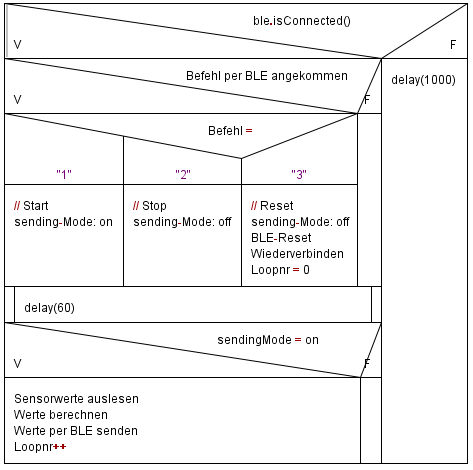
\includegraphics[width=0.9\textwidth]{images/k3-loopstructo.png}
	\caption {Struktogramm des Codeinhaltes der \texttt{loop()}-Methode}
	\label{fig:k3_loopstructo}
\end{figure}

Besteht keine BLE-Verbindung, wartet der Mikrocontroller 1000ms, bis er wieder mit dem erneuten Aufruf von \texttt{loop()} beginnt. Bei bestehender Verbindung wird zunächst eventuelle empfangene Befehle der Android-App ausgewertet. Sollen Daten gesendet werden (\texttt{Senden-Modus = on}), wird mit dem Auslesen der Sensor-Werte und dem Sende dieser per BLE fortgefahren. 

